\documentclass[11pt,titlepage]{article}
\usepackage[latin1]{inputenc}

\usepackage{hyperref}
\usepackage{amsmath}
\usepackage{long table}
\usepackage{amsfonts}
\usepackage{amssymb}
\usepackage{graphicx}
\usepackage{textcomp}
\author{Nicholas Bonham and Roy Smart}
\title{EGSE Software \\ A Guide to the Source}
\date{\today}

\setlength{\textwidth}{14.5cm}


\begin{document}
	
\maketitle
\tableofcontents
\newpage
	
\section[Revisions]{Revision History}
	\begin{longtable}{|c|c|r|r|}
		\hline
		Revision	&	Date	&	\multicolumn{1}{c|}{History}	&	\multicolumn{1}{c|}{Initial}\\
		\hline
		0.1		&	06-05-2017	&	Created	&	NPB\\
		\hline
	\end{longtable}
	
\newpage

\section{Introduction}
\hrulefill
\\
	In the summer of 2018, the Kankelborg research group will launch a sounding rocket containing the instruments ESIS and MOSES. Each instrument is designed to image the sun in the Extreme Ultraviolet wavelengths. In order to communicate with the instrument and send commands to and from the instrument during flight, a flight software that operates rapidly needs to be implemented. This flight software is controlled from the ground and sends commands to the instrument via an RS-232 radio connection. \par
	The EGSE server and client are programs written in Java and will be run on EGSE 2, a computer running Linux Mint 17 in the EGSE tower. The EGSE tower consists of multiple computers which run different programs in order to communicate with the instrument as well as display data sent back to the ground. The server and client are used to exchange HLP packets with the flight computer while the instrument is on the ground. The flight computer will be interfaced with EGSE 2 via an Ethernet connection. \par
	The existing EGSE software was written by Matthew Handley with contributions from Roy Smart, Jackson Remington, and David Keltgen. While the existing software was successful, updates were necessary due to the changes in the payload. Rather than sending only the MOSES instrument, ESIS will also be in the payload. The two instruments will be sharing the same up-link interface. To ensure successful communication between the flight computer and both instruments, modifications to multiple sections of the EGSE software were required. \par

\newpage

\section{EGSE Server}
\hrulefill
\\
The EGSE server is operated through a graphical user interface (GUI) that contains a slew of panels corresponding to different functions of the EGSE server. The primary function of the server is a gateway for communication between the EGSE client and the MOSES instrument.
\begin{figure}[h]
	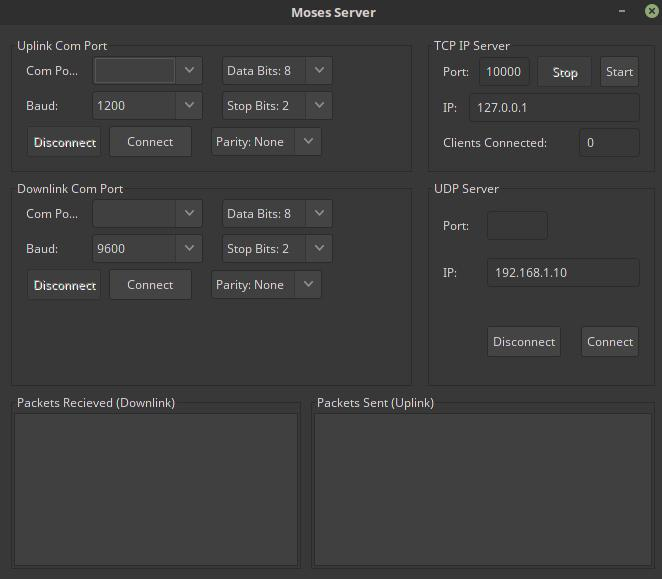
\includegraphics[width=\textwidth]{EGSE_server_image}
	\caption{Screenshot of the EGSE Server GUI.}
\end{figure}


	\subsection{Uplink/Downlink Com Port}
	\hrulefill
	\\
	The Uplink and Downlink Com port panels are designed to detect port interfaces and control the data flow rate, size, and stop bit size. When a port is active, it is displayed as an option that can be selected in the drop-down box. The baud rate drop-down box contains a number of baud rates that can be selected. Baud rate is defined as the rate information is being relayed in a communication channel. Once all of the options are configured appropriately, the \texttt{Connect} button establishes the connection to the specified port location.

	\subsection{TCP IP Server}
	\hrulefill
	\\
	The TCP IP server is responsible for relaying information sent as TCP packets. This panel gives the user the ability to specify which port and IP address will be used for TCP packets transmission. The \texttt{Start} button initiates the connection; the \texttt{Stop} button terminates this connection. The \texttt{Clients Connected} window displays the number of successful connections to the specified port and IP address.
	
	\subsection{UDP Server}
	\hrulefill
	\\
	The UDP server is responsible for linking a connection for UDP packets to be transmitted. These packets are identical to the commands being sent to the server from the EGSE client, but are transmitted as UDP packets, rather than TCP packets. The UDP port is specified in the \texttt{Port} text field. The IP address to be sent to is specified in the \texttt{IP} text field. \par
	
	
	\subsection{Packets Received/Sent Windows}
	\hrulefill
	\\
	The windows at the bottom of the EGSE server display the packets of information that are either being sent or received by the server.	

\newpage
\section{EGSE Client}
\hrulefill
\\

	\subsection{Timer}
	\hrulefill
	\\
	
	\begin{figure}[h]
		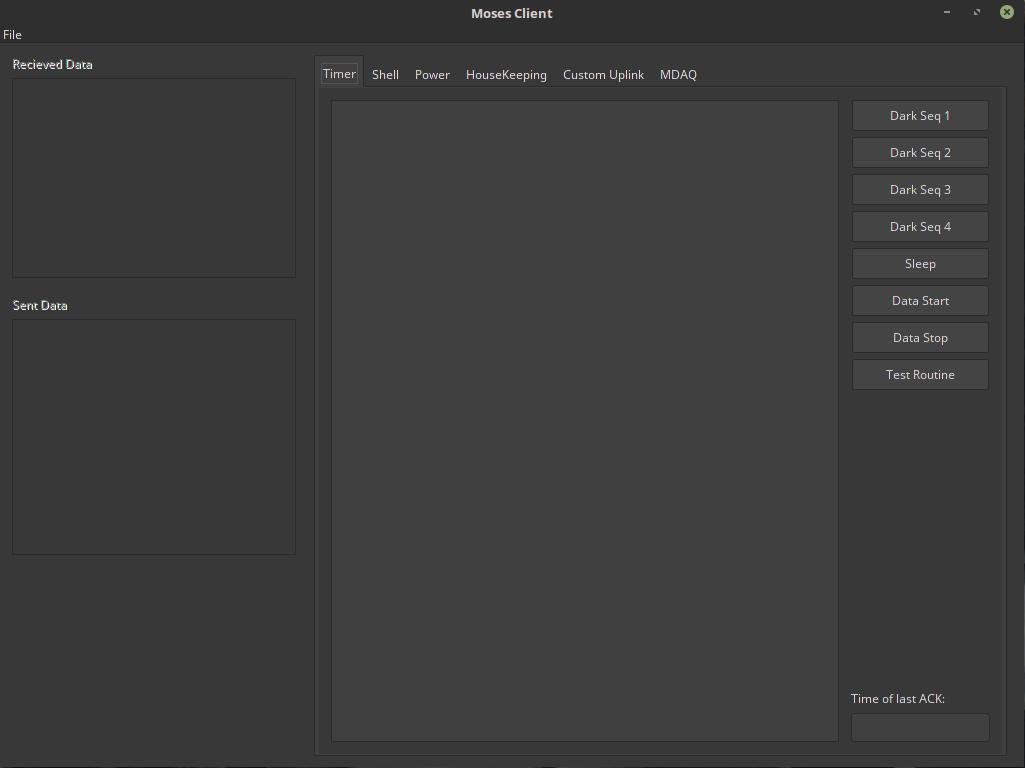
\includegraphics[width=\textwidth]{EGSE_client_image}
		\caption{Screenshot of the EGSE Client GUI.}
	\end{figure}
	
	The timer tab in the EGSE client is a section in which the user may send timing commands to the EGSE server, and then to the instrument. The timing commands are as follows:
	\begin{enumerate}
		\item \texttt{Dark Seq 1-4}: These links instruct the MOSES flight computer to begin the dark sequence time line which records exposures from the CCDs in the instrument. These sequences take multiple exposures with the shutter closed at varying exposure lengths. This is a necessary task in order to model the dark current from the ROE. Dark sequences are taken at various stages of the mission including while the instrument is on the ground, during the up-leg of the flight, and after the instrument records data with an open shutter. A fourth dark sequence is an optional feature that may be necessary based on the user's discretion.
		\item \texttt{Sleep}: This instructs the flight computer to go into sleep mode, which shuts off some of the components of MOSES until they are needed again.
		\item \texttt{Data Start}:
		\item \texttt{Data Stop}:
		\item \texttt{Test Routine}: The test routine effectively pings the flight computer to make sure that it is communicating with the EGSE software. 
	\end{enumerate}

	\newpage
	\subsection{Shell}
	\hrulefill
	\\
	
	\begin{figure}[h]
		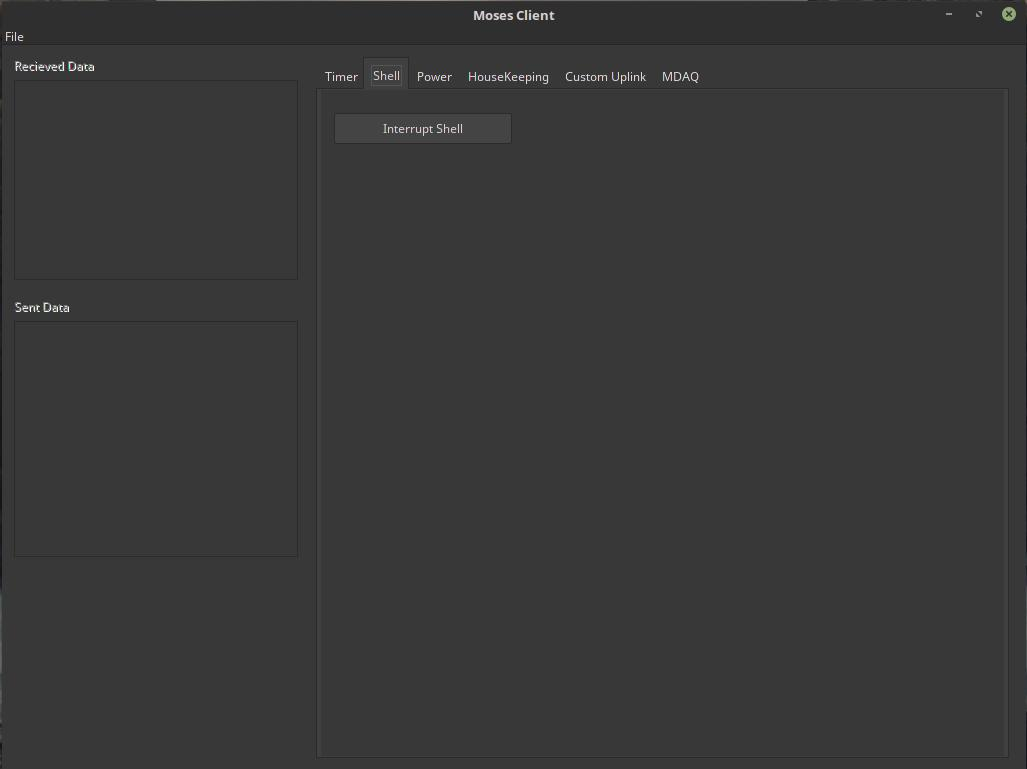
\includegraphics[width=\textwidth]{EGSE_client_shell}
	\end{figure}

	Sometimes, it is necessary to terminate a process, such as if the process is stuck in a loop, or if you suddenly realize you accidentally typed a very dangerous linux command! The \texttt{Interrupt Shell} button allows the current process to stop running on the shell. 

	\newpage
	\subsection{Power}
	\hrulefill
	\\
	
		\begin{figure}[h]
		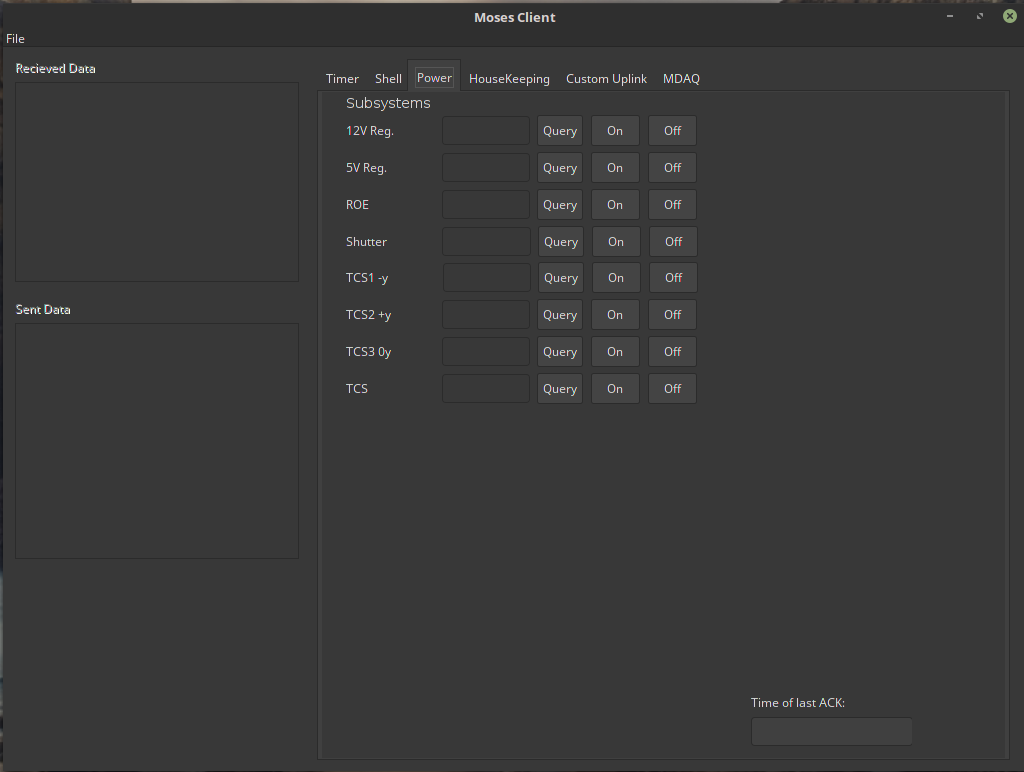
\includegraphics[width=\textwidth]{EGSE_client_power}
		\end{figure}
	
	The power tab contains commands for the power subsytems. The \texttt{On} button turns a specific system on. Likewise, the \texttt{Off} button turns a specific system off. Each of the electrical components on the instrument can be controlled from here. The purpose of each electrical system is as follows:
	\begin{enumerate}
		\item \texttt{12V Reg.}: The 12 V regulated supply powers many components of the instrument, including...
		\item \texttt{5V Reg.}: The 5 V regulated supply powers...
		\item \texttt{ROE}: The read out electronics for the CCDs in the MOSES instrument. These record voltage values corresponding to intensity measurements which form an image. The ROE contains an analog-digital converter allowing the data to be saved and accessible later on.
		\item \texttt{Shutter}: The shutter allows light to pass through the instrument. Once the shutter power system is turned on, the shutter can be opened, allowing MOSES to record data.
		\item \texttt{TCS1 -y}:
		\item \texttt{TCS2 +y}:
		\item \texttt{TCS3 0y}:
		\item \texttt{TCS}:
		
	\end{enumerate}
	

	
	\newpage
	\subsection{Housekeeping}
	\hrulefill
	\\
	
	\begin{figure}[h]
		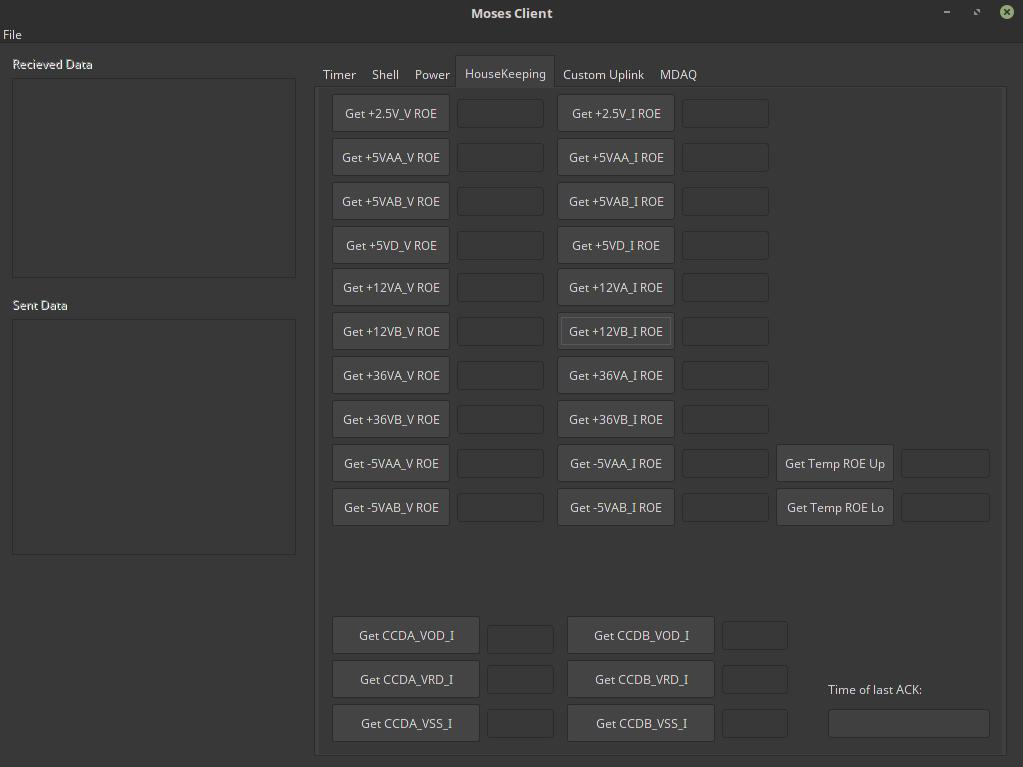
\includegraphics[width=\textwidth]{EGSE_client_housekeeping}
	\end{figure}
	
	\newpage
	\subsection{Custom Uplink}
	\hrulefill
	\\
	
	\begin{figure}[h]
		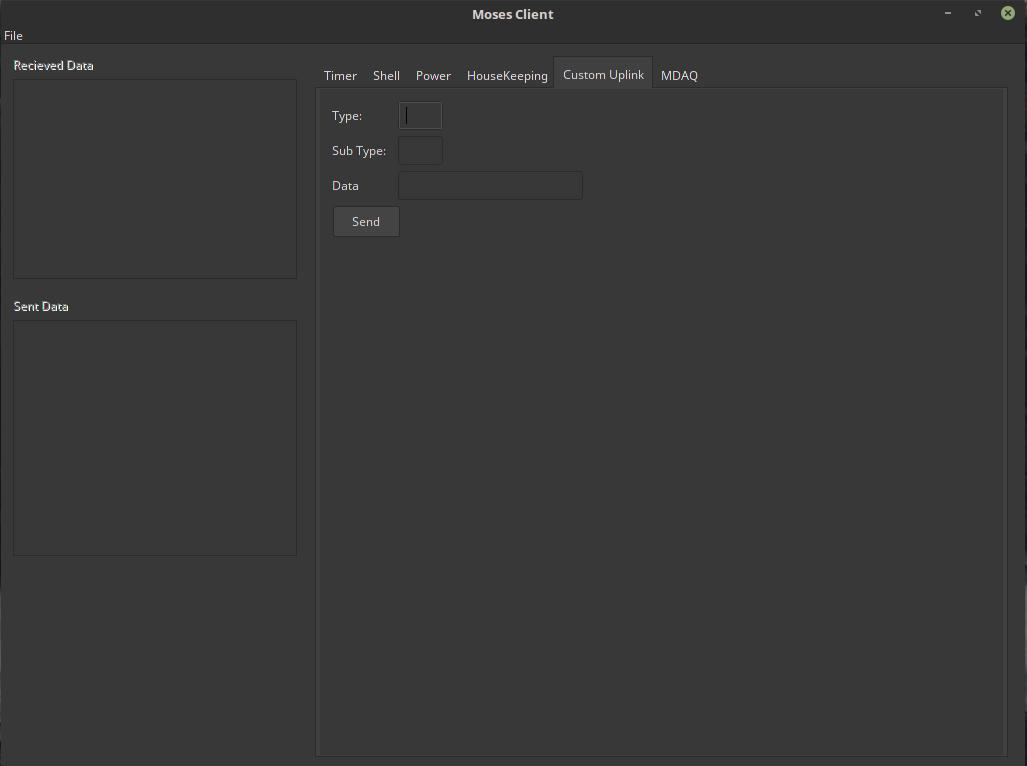
\includegraphics[width=\textwidth]{EGSE_client_custom_uplink}
	\end{figure}
	
	\newpage
	\subsection{MDAQ}
	\hrulefill
	\\
	
	\begin{figure}[h]
		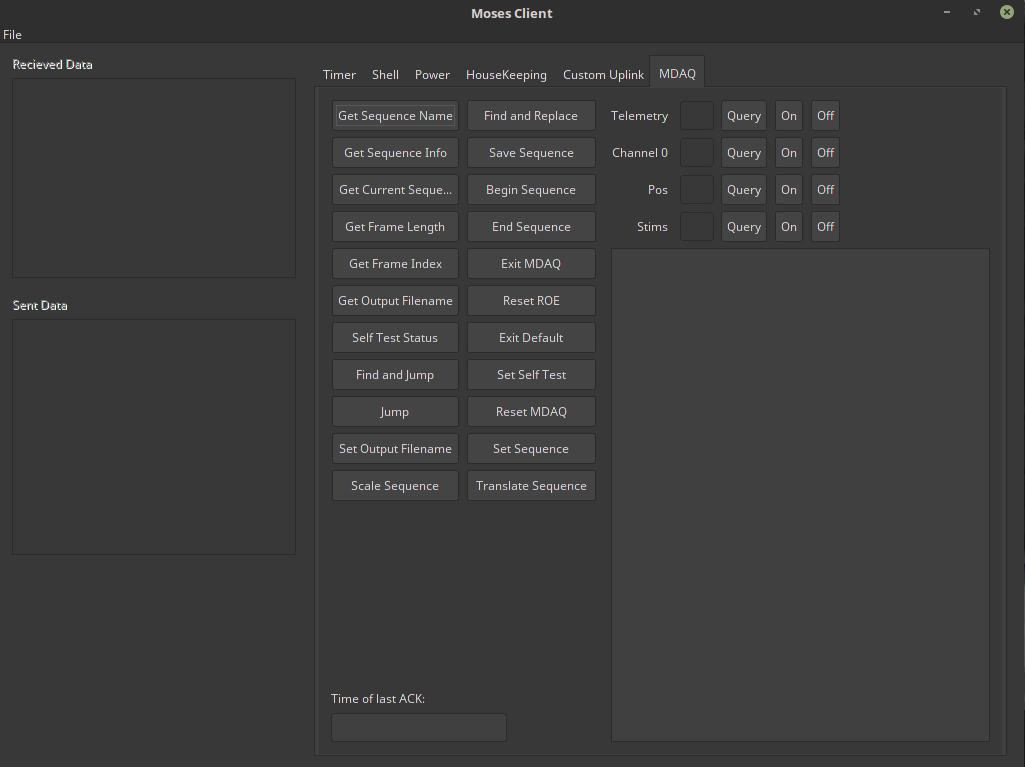
\includegraphics[width=\textwidth]{EGSE_client_mdaq}
	\end{figure}
	
\newpage	
\section{Setup}
	\subsection{Operation}
	\hrulefill
	\\
	In order to startup the EGSE software, both the EGSE server and EGSE client need to be started. This can be done through an IDE such as NetBeans, or may be done through the command line in the terminal. Once those are up and running, the TCP transmission on the EGSE server must be initiated. This is done by clicking \texttt{Start} under the TCP IP Server panel on the server. Make sure the appropriate port and IP address are specified. \par
	To connect the client to the server, go to \texttt{File} and click \texttt{Connect}. This selection will bring up a ne window with options for connecting to a specific port and IP address. These must match the specified port and address on the server. A successful connection will print, "Connected to $\langle$IP address$\rangle$:$\langle$port$\rangle$". Conversely, an attempt to connect to the server before starting the server, or typing a mismatch in the port or IP fields will result in an error message, "Couldn't get I/O for the connection to: $\langle$IP address$\rangle$:$\langle$port$\rangle$". \par
	Once a successful connection is established, the communication between the server and client may commence. To terminate the connection, press the \texttt{Stop} button in the TCP IP Server panel. This will print, "TCP socket closed". 
	\\
	
\newpage
\section{Dictionary of Abbreviations}
	\hrulefill
	\\
	\begin{enumerate}
		\item EGSE - Electronic Ground Station Equipment
		\item MOSES - Multi-Order Slit-less EUV Spectrograph
		\item ESIS - EUV Snapshot Imaging Spectrograph
		\item HLP - Housekeeping Link Protocol
		\item TCP - Transmission Control Protocol
		\item UDP - User Datagram Protocol
		\item CCD - Charge-Coupled Device
		\item ROE - Readout Electronics
		\item MDAQ - Mission Data Acquisition
	\end{enumerate}

	
\end{document}